%%%%%%%%%%%%%%%%%%%%%%%%%%%%%%%%%%%%%%%%%%%%%%%%%%%%%%%%%%%%%%%%%%%%%%%%%%%%%%%%
%2345678901234567890123456789012345678901234567890123456789012345678901234567890
%        1         2         3         4         5         6         7         8

\documentclass[conference]{IEEEtran}
\usepackage{times}

% Subfiles package
%\usepackage{subfiles}

% References
\usepackage[numbers]{natbib}

% Usual setup packages
\usepackage{listings} % For including source code with highlighting
\usepackage{hyperref} % For better hyper-link integration
\usepackage[bottom]{footmisc} % places footnotes at page bottom

% Packages for verbatim text blocks
\usepackage{alltt} % Package for including math in verbatim text
\usepackage{fancyvrb}

% Packages for math symbols and other mathey things
\usepackage{amsthm}
\usepackage{amsmath}
\usepackage{amsfonts}
\usepackage{amssymb}

% Packages for including pseudo-code
\usepackage{algorithmicx}
\usepackage{algorithm}
\usepackage{algpseudocode}

% Packages that handle tables, figures and other floats
\usepackage{tabularx}
\usepackage{multirow}
\usepackage{float} % To make floats movable
\usepackage{subcaption}
\usepackage[table]{xcolor}

% Packages for drawing graphs, FSMs, etc.
\usepackage{pgf}
\usepackage{tikz}
\usetikzlibrary{shapes,arrows,calc,fit,positioning,shapes.symbols,shapes.callouts,patterns,automata,matrix}

% Remove red boxes around refs
\hypersetup{
    colorlinks,
    citecolor=black,
    filecolor=black,
    linkcolor=black,
    urlcolor=blue
}

% ------------------------------ CUSTOM MACROS ------------------------------------
% Nice little macro for adding a comment box. Include incrementing comment numbers.
\newcounter{comcount}
\setcounter{comcount}{0}
\newcommand{\mycomment}[1]
{
\refstepcounter{comcount}
\smallskip\noindent\fbox{\parbox{\linewidth}{\emph{Comment \arabic{comcount}} : \small{#1}}} 
}

\DeclareMathOperator*{\argmin}{\arg\!\min\>}
\newcommand{\amin}[1]{\underset{#1}\argmin}
\DeclareMathOperator*{\argmax}{\arg\!\min\>}
\newcommand{\amax}[1]{\underset{#1}\argmax}

\newcommand{\sig}{\mathcal{S}}
\newcommand{\ceil}[1]{\lceil#1\rceil}
\newcommand{\xm}{x_{\hat{m}}}

\begin{document}
\title{Modeling Collaborative Swarming Behavior as a Global Game}
\author{Author Names Omitted for Anonymous Review. Paper-ID [add your ID here]}

\maketitle

%%%%%%%%%%%%%%%%%%%%%%%%%%%%%%%%%%%%%%%%%%%%%%%%%%%%%%%%%%%%%%%%%%%%%%%%%%%%%%%%
\begin{abstract}
Abstract goes here\ldots
\end{abstract}

\IEEEpeerreviewmaketitle

%%%%%%%%%%%%%%%%%%%%%%%%%%%%%%%%%%%%%%%%%%%%%%%%%%%%%%%%%%%%%%%%%%%%%%%%%%%%%%%%
\section{Introduction}\label{sec:intro}
Collaborative tasks are an important set of scenarios often studied in the field of swarm robotics. Many of the tasks we envision teams of robots performing, such as object transport \cite{sugawara2012}, oil-spill containment\cite{beni2005swarm}, firefighting\cite{krishnanand2006glowworm}, pattern recognition \cite{beni1993swarm}, and cooperative surveillance fall under this broad umbrella of collaborative tasks. While considerable work has been done in studying the specific details of particular tasks in the above list, the more general question of estimating a team size appropriate for the size of the task remains largely unanswered. It is generally assumed that a required team size is provided by a domain expert before a collaborative task is attempted by the robots. But, as is often the case with teams of humans attempting a collaborative task, this number not easy to guess, e.g., When trying to lift and move a heavy object, it is difficult to estimate how many people will be required. A number of factors such as the mass and dimensions of the object, and the length and complexity of the path (perhaps involving staircases) come into play when deciding this number. Therefore, there exist a range of team sizes that may accomplish this task to varying degrees of success.

\begin{figure*}[!ht]
\centering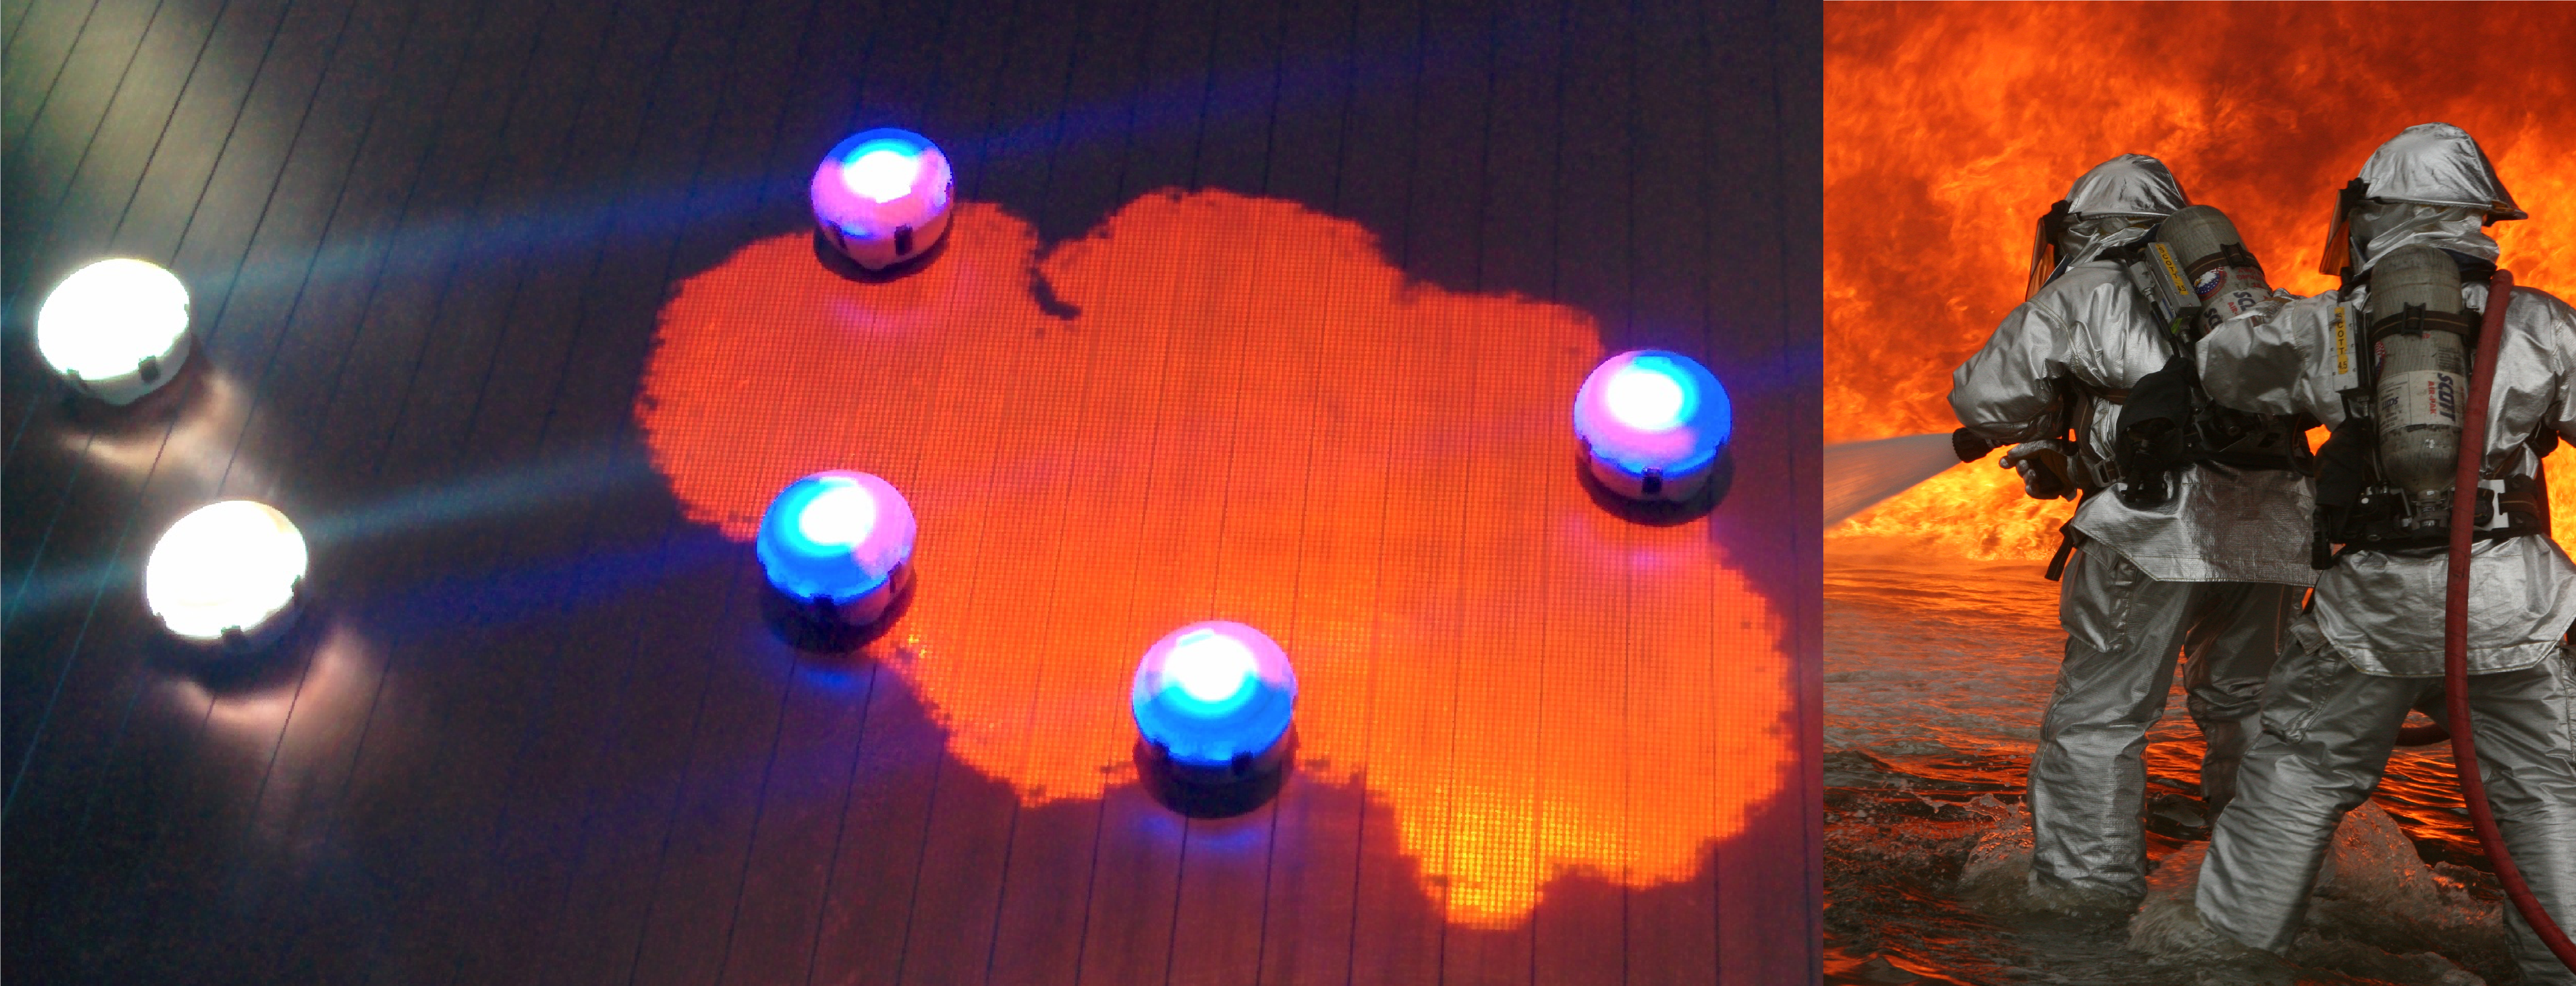
\includegraphics[width=\textwidth]{../figures/dropletfire.png}
\centering\caption{}\label{fig:dropletfire}
\end{figure*}

The goal of this paper is to model and analyze such tasks that have the property of \emph{concurrent benefit} using the concept of global games from the field of game theory. We define concurrent benefit as an attribute of a collaborative task wherein the exact number of agents required to successfully complete the task is unknown and varies with time. The probability of success depends, non-linearly, on the average number of agents assigned to that task. For example, in a firefighting scenario (see Fig.~\ref{fig:dropletfire}), a single robot trying to contain a large fire will likely be unsuccessful on its own (and will waste fire retardant in trying) but a group of robots within a certain group size range may be able to contain the flames to a reasonable level of success. This measure of success is related non-linearly to the group size, i.e. where 5 or even 10 robots have a negligible effect on containing the fire, perhaps 12 or more very quickly become capable of succeeding in the task.



\begin{figure}[!ht]
\centering\includegraphics[width=\columnwidth]{../figures/sigmoid1.png}
\centering\caption{}\label{fig:sigmoid}
\end{figure}

Collaborative tasks can be modeled as a global game with multiple players/agents. All tasks take place in a large operational area. Tasks or collaboration sites appear within the operational area at random. All agents are dispersed uniformly and at random within the operational area. The reader should note that the method of searching for a collaboration site is arbitrarily chosen for the purposes of the model discussed in this paper; in practice, any search pattern or algorithm that best fits the scenario may be chosen without affecting the conclusions provided by our model. Once an agent arrives at a collaboration site, it independently makes an estimate, $\tau$, for the group size required to successfully complete the task at that site. This estimate is derived from an estimation function, $\Xi(\cdot)$, that takes in a noisy signal, $x$, as input. $\Xi(x)$ quantifies the size and complexity of the presented task using the robot's sensors and internal state information. This is analogous to a human assessing a situation using their senses and other domain specific data provided to him. The reason for using an estimation function is discussed in Section\ref{sec:ggresults} of this paper.

\begin{figure}[!ht]
\centering\includegraphics[width=\columnwidth]{../figures/globalgamesetup.png}
\centering\caption{}\label{fig:ggsetup}
\end{figure}

The noisy signal $x$ is a sum of two terms, $x = \theta + \epsilon$, where $\theta$ is considered the \emph{ground truth} signal and $\epsilon$ is a Gaussian noise term with mean $0$ and standard deviation $\sigma$, as seen in Fig.~\ref{fig:ggsetup}. This setup helps situate this multi-robot collaboration model in a global game setting. The \emph{player} terminology often used in game theory literature maps directly to robots (or agents) in swarm robotics. Each player/agent makes independent algorithmic decisions and overall system equilibrium conditions are measured via the set of joint actions between agents. A brief overview of the theory of global games is provided in Section \ref{sec:ggoverview}.

\subsection{Related Work}\label{subsec:rw}



\section{Global Games: A Brief Overview}\label{sec:ggoverview}




\section{Results from Game Theory}\label{sec:ggresults}



\section{Experiment Setup}\label{sec:expsetup}
We ran collaborative task completion experiments with the \emph{Droplet} swarm robot platform to validate results presented in the previous section. The experiment employs they robots' overhead RGB sensors to simulate a fire that is projected down onto the arena using a standard off-the-shelf projector. The goal of the experiment is to have the robots collaboratively put out these projected fires by congregating at the perimeter of the fire and turning on their blue LEDs together. The projected fires increase in size and intensity (indicated by changing color from the red to the yellow spectrum) with time.


\section{Experimental Results}\label{sec:expresults}




\section{Discussion}\label{sec:disc}




\section{Conclusion}\label{sec:conc}




%%%%%%%%%%%%%%%%%%%%%%%%%%%%%%%%%%%%%%%%%%%%%%%%%%%%%%%%%%%%%%%%%%%%%%%%%%%%%%%%
%%%%%%%%%   The Bibliography, if any   %%%%%%%%%
\bibliographystyle{plainnat}		% or "siam", or "alpha", etc.
\bibliography{../refworks}
\end{document}